%!TeX root=../control_rapido.tex
%!TeX spellcheck = es_ES 

\chapter{Métodos de control PID}


Durante esté capítulo se tratará un ejemplo de control de velocidad (\textbf{Cruise Control}). Se mostrará al lector la base de control continuo para despues explicar temas relacionados a \textbf{control robusto}.

\begin{figure}[h!]
	\centering
	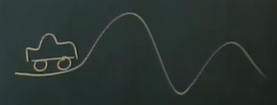
\includegraphics[width=0.4\linewidth]{fig/cruisecontrol}
	\caption{Un automovil necesita tomar en cuenta entradas exógenas como cerros, incertidumbres del modelo y perturbaciones para mantener una velocidad constante.}
	\label{fig:cruisecontrol}
\end{figure}

Un modelo a lazo abierto tiene un controlador de la forma 
\[
\Cu = \MK \Cr
\]
donde $\MK$ es la ganancia del controlador y $\Cr$ es la actuación.

Imaginemos el caso del automovil. Tenemos un sistema SISO (single input, single output), $u$ siendo la potencia erogada por el motor (y los frenos) que es controlada por un actuador. Supongamos que la velocidad es determinada por el input según $y=2u$. Es decir, si queremos una velocidad $y_0$, precisamos la mitad del valor de $y_0$ en actuación para llegar. Si $r$ es el valor de $y$ que se desea llegar, $u_{\openloop}=\frac{1}{2}r$ para un controlador a lazo abierto (LA). 

\begin{figure}[htb!]
	\centering
	\begin{tikzpicture}[auto, node distance=2cm]
		\node[block, label=above:Sistema automovil] (sys) {$y=2u$};
		\node[input,left of=sys,label=below:pot./freno] (in) {};
		\node[block,left of=in] (con) {Controlador};
		\node[input,left of=con,label=below:$y$ deseado] (conin) {};
		\node[output, right of=sys,label=below:velocidad] (out) {};
		\draw[->] (con)-- (in) -- node[above] {$u$} (sys);
		\draw[->] (sys) -- node[above] {$y$} (out);
		\draw[->] (conin) -- node[above] {$r$} (con);
	\end{tikzpicture}
	\caption{Sistema a lazo abierto. Un auto imaginario en buenas condiciones toma una velocidad de dos veces la entrada.}
\end{figure}

Pero puede suceder que se esté intentando controlar un automóvil en condiciones precarias. Si los inyectores no se han limpiado desde hace décadas, tiene ruedas desinfladas, cilindros desgastados, puede suceder que para una entrada $u$ la velocidad sea $y=u$. A lazo abierto nuestro auto anda a mitad de la velocidad de la que se le pide! No es todo, las perturbaciones tendrán un efecto acumulado sobre las incertezas, representadas con $d$. El modelo real del automóvil será diferente al del lazo abierto 

\[
u_\openloop = \frac{r}{2}, \qquad y_{\true} = u + d, \qquad y_\openloop = \frac{r}{2} + d
\]

Como ya habremos visto, los sistemas a lazos cerrados nos dan los beneficios de estabilidad, manejo de incertezas y perturbaciones. La figura \ref{fig:closedloopcruisecontrolexample} implementa un control a lazo cerrado para tal fin.
\begin{figure}[htb!]
	\centering
	\begin{tikzpicture}[auto, node distance=2cm]
	% We start by placing the blocks
	\node [input, name=input] {};
	\node [sum, right of=input] (sum) {};
	\node [blck, right of=sum,label=below:Controlador] (controller) {$K$};
	\node [block, right of=controller,
	node distance=3cm,label=below:Sistema] (system) {$P$};
	\node [sum, right of=system, node distance=2cm,  pin={[pinstyle]above:$d$}] (dist) {};
	\node [output, right of=dist] (output) {};
	
	\draw [->] (controller) -- node[name=u] {$u$} (system);
	\coordinate [below of=u] (tmp);
	\draw [->] (input) -- node {$r$} (sum);
	\draw [->] (sum) -- node {$\error$} (controller);
	\draw [->] (system) -- (dist);
	\draw [->] (dist) --  node [name=y] {$y$}(output);
	\draw [->] (y) |- (tmp) -| node[pos=0.99] {$-$} 
	node [near end] {$y$} (sum);
	\end{tikzpicture}
	\caption{Sistema a lazo cerrado con control proporcional.}
	\label{fig:closedloopcruisecontrolexample}
\end{figure}

En el sistema de la figura aparece el error $\error$ que resulta ser la resta $\error = r-y\closedloop$.

Ahora las ecuaciones que describen el sistema serán
\begin{IEEEeqnarray*}{c}
u_\closedloop = K\error = K(r-y)  \\
y_\closedloop = Pu +d 
\end{IEEEeqnarray*}

Sustituyendo se llega a que $y_\closedloop = PKr - PKy_\closedloop + d$. Resolviendo para $y_\closedloop$
\begin{IEEEeqnarray*}{c}
y_\closedloop = \underbrace{\frac{PK}{1+PK}}_{\text{I}}r + \underbrace{\frac{1}{1+PK}}_{\text{II}}d
\end{IEEEeqnarray*}

El término I nos dice que tan bien la salida $y_\closedloop$ se iguala a $r$ (el valor deseado de $y$). El término II nos dice que tanto las perturbaciones son reducidas por el lazo de control. Recuerde que lo que queremos es que $y_\closedloop=r$, esto se puede lograr aumentando $K$ para que el término I se iguale a 1 y el término II se vaya a cero. Tal vez le resulte escandaloso al lector que con un lazo tan simple el aumento de $K$ indiscriminado mejore el rechazo de perturbaciones y convergencia a $r$, es importante saber que no viene sin sus desventajas.

Desventajas de control proporcional
\begin{itemize}
	\item $K$ esta limitado por el actuador de la realidad. No podemos esperar que el automovil consuma 10 litros de nafta en 1 segundo para llevar $y$ a $r$.
	\item Retardo en la medición puede ocasionar inestabilidad/oscilaciones si $K$ es muy grande. Incertidumbres del sistema también pueden ser nocivas con el aumento de $K$.
	\item En la ausencia de perturbaciones siempre va haber un pequeño error en régimen estacionario. Esto se debe a que el término I llega cerca pero nunca es igual a 1. Ejemplo: Para $PK=100$ va haber un error estacionario del $1\%$. Para remediar esto se puede implementar un integrador
\end{itemize}

\section{Control Integrador}

\begin{figure}[htb!]
	\centering
	\begin{tikzpicture}[auto, node distance=1.5cm]
		\node [block ,label=below:Sistema] (sys) {$P$};
		\node [input, name=sysin, left of=sys] {};
		\node [sum, left of=sysin] (syssum) {+};
		\coordinate[left of=syssum] (gainaux) {};
		\node [blck, above of=gainaux,label=below:Proporcional] (prop) {$K_P$};
		\node [blck, below of=gainaux,label=below:Integrador] (int) {$K_I\, \int$};
		\coordinate [left of=gainaux] (error);
		\node [sum, left of=error, node distance=1cm] (errorsum) {};
		\node [input, left of=errorsum] (rin) {};
		\node [sum, right of=sys,pin={[pinstyle]above:$d$}, node distance=2cm] (dist) {};
		\node[output, right of=dist] (out) {};
		\coordinate [below of=int] (feedback);
		
		\draw [->] (errorsum) -- node {$\error$} (error) |- (prop);
		\draw [->] (prop)  -| (syssum);
		\draw [->] (error) |- (int);
		\draw [->] (int)  -| (syssum);
		\draw [->] (syssum) -- node {$u$} (sys);
		\draw [->] (sys) -- node[pos=.99] {$+$} (dist);
		\draw [->] (dist) -- node[name=y] {$y$} (out);
		\draw [->] (y) |- (feedback) -| node[pos=.99] {$-$} node [near end] {$y$} (errorsum);
		\draw [->] (rin) -- node {$r$} (errorsum);
	\end{tikzpicture}
	\caption{Sistema a lazo cerrado con control proporcional.}
	\label{fig:picontroller}
\end{figure}


La ley de control para el sistema de la figura \ref{fig:picontroller}
\begin{IEEEeqnarray*}{c}
u(t) = K_P(r-y)  + K_I \overbrace{\int_0^t (r-y)\diff \tau}^{=z}
\end{IEEEeqnarray*}

Las integrales en sistemas de control tienen la función de guardar en memoria el los estados anteriores del sistema. Se requiere entonces armar una ecuación auxiliar para cada integral

\begin{IEEEeqnarray*}{c,l}
\dot{x} &= -x -K_Px + K_Iz + K_P r\\
\dot{z} &= r - x \\
u &= K_P (r-x) + K_I z
\end{IEEEeqnarray*}

Las ecuaciones del controlador quedarían en forma matricial
%\todo{Segun un comentario el -1 de la segunda fila primera columna deberia ser positivo...}
\begin{IEEEeqnarray*}{c,l}
\frac{\diff}{\diff t} \begin{bmatrix}
x \\ z
\end{bmatrix} &=
\begin{bmatrix}
-1-K_P& K_I \\
-1 &  0 
\end{bmatrix} 
\begin{bmatrix}
x \\ z
\end{bmatrix}
+
\begin{bmatrix}
K_P \\
1
\end{bmatrix} r \\
y &= \begin{bmatrix}
1 & 0
\end{bmatrix}
\begin{bmatrix}
x \\ z
\end{bmatrix}
\end{IEEEeqnarray*}

Lo que hemos aprendido es que aumentando el espacio de variables con una variable $z$ para el integrador e implementandolo en el lazo de control podemos reducir el error en régimen estacionario a 0 y además converger más rápido a $r$.




\section{Sensibilidad y sensibilidad complementaria}

\begin{figure}[htb!]
	\centering
	\begin{tikzpicture}[auto, node distance=1.5cm]
	\node [block ,label=below:Sistema] (sys) {$\MP$};
	\node [input, name=sysin, left of=sys] {};
	\node [blck, left of=sysin] (con) {$\MK$};
	\coordinate [left of=con] (error);
	
	\node [sum, left of=error, node distance=1cm] (errorsum) {};
	\node [input, left of=errorsum] (rin) {};
	\node [sum, right of=sys, node distance=2.5cm] (dist) {};
	\node [blck, above of=dist,pin={[pinstyle]above:$\Cd$}] (distmat) {$\MP_d$};
	\node[output, right of=dist] (out) {};
	\node [sum,below of=sys,
	pin={[pinstyle]below:$\Cn$}, node distance=2.2cm] (noise) {};
	\node [boxin,label=above:{Lazo $\ML=\MP\MK$}, fit=(sys) (con)] (box) {};
	
	\draw [->] (errorsum) -- node {$\error$} (error) -- (con);
	\draw [->] (con)  -- node {$\Cu$} (sys);
	\draw [->] (sys) -- node[pos=.99] {$+$} (dist);
	\draw [->] (dist) -- node[name=y] {$\Cy$} (out);
	\draw [->] (distmat) -- (dist);
	\draw [->] (y) |- node[pos=.99] {$+$} (noise) -| node[pos=.99] {$-$} node [near end] {$\Cy_m$} (errorsum);
	\draw [->] (rin) -- node {$\Cr$} (errorsum);
	\end{tikzpicture}
	\caption{$\Cy_m$ es el vector de mediciones el cual es afectado por el ruido $\Cn$.}
	\label{fig:loopdaloop}
\end{figure}


La función de transferencia del lazo $\ML=\MP \MK$ va ser el sujeto de estudio. Cuando se trabaja con transferencias es importante el orden de multiplicación. Como indica la figura, la primer función de transferencia en actuar (en el caso del lazo, $\MK$) va estar al final del producto. Ya no estamos hablando de escalares tampoco, estas funciones de transferencia son matrices que operan sobre vectores de error, entrada y perturbaciones.

El objetivo de la realimentación es 

\begin{description}
	\item[Diseñar] estabilidad
	\item[Compensar] incertidumbre del sistema
	\item[Rechazar] perturbaciones
	\item[Atenuar] ruido
\end{description}

El controlador, específicamente, la transferencia $\MK$ estará encargada de que al error $\error$ no le lleguen ruido, perturbaciones.

De la figura \ref{fig:loopdaloop} se obtiene
\begin{IEEEeqnarray*}{c}
\Cy_m=\eye \Cy_m = \MP_d \Cd + \MP \MK \overbrace{(\Cr - \Cy_m - \Cn)}^{=\error} \\
\left(\eye+ \MP\MK\right)\Cy_m = \MP \MK \Cr + \MP_d \Cd \\
\Cy_m = \underbrace{\left(\eye + \MP\MK\right)^{-1} \MP \MK}_{\text{I}} \Cr + \underbrace{\left(\eye + \MP\MK\right)^{-1}}_{\text{II}} \MP_d \Cd- \underbrace{\left(\eye + \MP\MK\right)^{-1} \MP\MK}_{\text{III}} \Cn
\end{IEEEeqnarray*}

Durante el curso de los próximos capítulos se va querer diseñar una ganancia $\MK$ para que: el término I sea cercano a 1 así podemos rastrear la referencia con poco error a bajas frecuencias, el término II sea pequeño para frecuencias donde esperamos perturbaciones, y que el término III sea pequeño para frecuencias donde esperamos obtener ruido (probablemente a altas frecuencias).

El término II se llama la transferencia de sensibilidad \eqref{eq:sensitivity} e indica que tan sensible es el vector salida $\Cy$ a las perturbaciones. El término $\left(\eye + \MP\MK\right)^{-1} \MP \MK$ es la sensibilidad complementaria \eqref{eq:sensitivityCompl} que es asociada a la referencia y al ruido.
\begin{IEEEeqnarray*}{c,l}
\ML &= \MP \MK \\
\MS &= \left(\eye + \ML\right)^{-1}\IEEEyessubnumber \label{eq:sensitivity} \\ 
\MT &= \left(\eye + \ML\right)^{-1} \ML \IEEEyessubnumber \label{eq:sensitivityCompl}
\end{IEEEeqnarray*}
una identidad demostrable con álgebra lineal que resulta de estas transferencias es 
\begin{IEEEeqnarray}{c}
\MS + \MT = \eye    \qquad \forall s \in \mathbb{C}
\end{IEEEeqnarray}

Lo más interesante de todo esto es la forma de representar el error a partir de la sensibilidad ya que es lo que se quiere reducir
\begin{IEEEeqnarray}{c}
\error = \Cr - \Cy_m = \MS\Cr - \MS \MP_d \Cd + \MT \Cn
\end{IEEEeqnarray}
lo deseable va ser elegir $\MS$ y $\MT$ de tal forma que $\MS$ rechaze perturbaciones a bajas frecuencias mientras que $\MT$ atenué ruido a altas frecuencias. Estas funciones podrían entonces tener la forma de la figura \ref{plt:bodeSensitivity}. Como $\MS$ y $\MT$ tienen que sumar uno hay una limitación importante al lazo que se puede diseñar.

\begin{figure}[htb!]
	\centering
	\begin{tikzpicture}[trim axis right]
	\begin{semilogxaxis}[bodeamp, ymin=-40,ymax=10,xmin=1e-2,xmax=1e2]
	\addplot[mark=none,red,ultra thick] table[x=x, y=bode, col sep=comma] {plots/bd_sensitivity.csv};
	\addlegendentry{$\MS$}
	\addplot[mark=none,blue] table[x=x, y=bode, col sep=comma, mark=none, red] {plots/bd_Csensitivity.csv};
	\addlegendentry{$\MT$}
	\addplot[mark=none,dotted,ultra thick] table[x=x, y=bode, col sep=comma, mark=none, black] {plots/bd_integrator.csv};
	\addlegendentry{$\ML$}
	\end{semilogxaxis}	
	\end{tikzpicture}
	\caption{Bode mostrando la sensibilidad para $L(s) = \frac{1}{s}$. La frecuencia de crossover  se encuentra en $\omega_c=1$ rad/s.}
	\label{plt:bodeSensitivity}
\end{figure}

Si quiero que a bajas frecuencias $\MS$ sea pequeño entonces necesito que $\ML$ sea muy grande a bajas frecuencias, de acuerdo con \eqref{eq:sensitivity}. Complementario a esto, si se quiere que a altas frecuencias se atenúe el ruido, $\ML$ tiene que ser bajo a estas frecuencias \eqref{eq:sensitivityCompl}. En fin, una función que cumple con esto es el integrador $\frac{1}{s}$ (y lo hace bien!). 

Un valor importante en el diseño del lazo el la \textbf{frecuencia de crossover} $\omega_c$. Por abajo de esta frecuencia las perturbaciones van a ser rechazadas y por arriba el ruido será atenuado. Si el lazo elegido es un integrador se puede definir $\omega_c$ según
\[
L(s)=\frac{\omega_c}{s}
\] 

Lo que veremos en los próximos capítulos es que la función $\MS$ nos da toda la información acerca de si el sistema va ser robusto o frágil. Veremos también como los picos en el bode de $\MS$ (como el que se vé en el gráfico \ref{plt:bodedampedmasssystem}) empeoran la sensibilidad y robustez del sistema


\begin{figure}[htb!]
	\centering
	\begin{tikzpicture}[trim axis right]
	\begin{axis}[grid=major, axis equal image, ylabel={Complejo}, xlabel={Real},legend pos=outer north east,]
	\addplot[mark=none,blue] table[x=real, y=imag, col sep=comma] {plots/nyq_dampedmass.csv};
	\addplot[red,mark=x] coordinates {(-1,0)};
	\addlegendentry{$G(i\omega)$}
	 \addplot [domain=0:2*pi,samples=50,dotted] ({.5419*sin((x)r)-1},{.5419*cos((x)r)});
	\end{axis}	
	\end{tikzpicture}
	\caption{Nyquist plot para la función transferencia del sistema masa-amortiguador-resorte. }
	\label{plt:nyq}
\end{figure}


